%%%%%%%%%%%%%%%%%%%%%%%%%%%%%%%%%%%%%%%%%
% Databases Report
%%%%%%%%%%%%%%%%%%%%%%%%%%%%%%%%%%%%%%%%%

%----------------------------------------------------------------------------------------
%	PACKAGES AND OTHER DOCUMENT CONFIGURATIONS
%----------------------------------------------------------------------------------------

\documentclass{article}

\usepackage{fancyhdr} % Required for custom headers
\usepackage{lastpage} % Required to determine the last page for the footer
\usepackage{extramarks} % Required for headers and footers
\usepackage[usenames,dvipsnames]{color} % Required for custom colors
\usepackage{graphicx} % Required to insert images
\usepackage{listings} % Required for insertion of code
\usepackage{courier} % Required for the courier font
\usepackage{enumitem}
\usepackage{titlesec}
\usepackage{url}
\usepackage{etoolbox}
\patchcmd{\thebibliography}{\section*{\refname}}{}{}{}

% Margins
\topmargin=-0.45in
\evensidemargin=0in
\oddsidemargin=0in
\textwidth=6.5in
\textheight=9.0in
\headsep=0.25in

\linespread{1.1} % Line spacing

% Set up the header and footer
\pagestyle{fancy}
\rfoot{Page\ \thepage\ of\ \protect\pageref{LastPage}} % Bottom right footer
\renewcommand\headrulewidth{0.4pt} % Size of the header rule
\renewcommand\footrulewidth{0.4pt} % Size of the footer rule

\setlength\parindent{0pt} % Removes all indentation from paragraphs

%----------------------------------------------------------------------------------------
%	CODE INCLUSION CONFIGURATION
%----------------------------------------------------------------------------------------

\definecolor{MyDarkGreen}{rgb}{0.0,0.4,0.0} % This is the color used for comments
\lstloadlanguages{Ruby}
\lstset{language=Ruby,
        frame=single, % Single frame around code
        basicstyle=\small\ttfamily, % Use small true type font
        keywordstyle=[1]\color{Blue}\bf, % Ruby functions bold and blue
        keywordstyle=[2]\color{Purple}, % Ruby function arguments purple
        keywordstyle=[3]\color{Blue}\underbar, % Custom functions underlined and blue
        identifierstyle=, % Nothing special about identifiers                                         
        commentstyle=\usefont{T1}{pcr}{m}{sl}\color{MyDarkGreen}\small, % Comments small dark green courier font
        stringstyle=\color{Purple}, % Strings are purple
        showstringspaces=false, % Don't put marks in string spaces
        tabsize=3, % 5 spaces per tab
        breaklines=true,
        morecomment=[l][\color{Blue}]{...}, % Line continuation (...) like blue comment
        numbers=left, % Line numbers on left
        firstnumber=1, % Line numbers start with line 1
        numberstyle=\tiny\color{Blue}, % Line numbers are blue and small
        %stepnumber=5 % Line numbers go in steps of 5
}

%----------------------------------------------------------------------------------------
%	DOCUMENT STRUCTURE COMMANDS
%----------------------------------------------------------------------------------------

\titlespacing\subsection{0pt}{1.0ex plus -1ex minus -.2ex}{-\parskip}
\setcounter{secnumdepth}{0} % Removes default section numbers
\newcounter{homeworkProblemCounter} % Creates a counter to keep track of the number of problems

\newcommand{\homeworkProblemName}{}
\newenvironment{homeworkProblem}[1][Question \arabic{homeworkProblemCounter}]{ % Makes a new environment called homeworkProblem which takes 1 argument (custom name) but the default is "Problem #"
\stepcounter{homeworkProblemCounter} % Increase counter for number of problems
\renewcommand{\homeworkProblemName}{#1} % Assign \homeworkProblemName the name of the problem
\subsection{\homeworkProblemName} % Make a section in the document with the custom problem count
}{}

\newcommand{\homeworkSectionName}{}
\newenvironment{homeworkSection}[1]{ % New environment for sections within homework problems, takes 1 argument - the name of the section
\renewcommand{\homeworkSectionName}{#1} % Assign \homeworkSectionName to the name of the section from the environment argument
}{}

%----------------------------------------------------------------------------------------
%	NAME AND CLASS SECTION
%----------------------------------------------------------------------------------------

\newcommand{\hmwkTitle}{Coursework\ \#3 \\\vspace{0.5in} \Huge{Report}} % Assignment title
\newcommand{\hmwkClass}{\LARGE COMS20700\ Databases} % Course/class
\newcommand{\hmwkDueDate}{ May\ 18,\ 2014} % Due date

%----------------------------------------------------------------------------------------
%	TITLE PAGE
%----------------------------------------------------------------------------------------

\title{
\vspace{0.2in}
\textmd{\textbf{\hmwkClass:\ \hmwkTitle}}\\
\vspace{0.5in}
\textmd{\hmwkDueDate}
\vspace{1.5in}
}

\author{
  \textbf{Liban Abdulkadir}\\
  \texttt{la12808@my.bristol.ac.uk}\\
  \textbf{Ana Dumitra\c{s}}\\
  \texttt{ad12461@my.bristol.ac.uk}\\
  \textbf{Andra Irimia}\\
  \texttt{ai12821@my.bristol.ac.uk}\\
  \textbf{Ioan Troan\v{a}}\\
  \texttt{it12754@my.bristol.ac.uk}\\
\vspace{1in}
}

\date{}

%----------------------------------------------------------------------------------------

\begin{document}

\maketitle

%----------------------------------------------------------------------------------------
%	TABLE OF CONTENTS
%----------------------------------------------------------------------------------------

%\setcounter{tocdepth}{1} % Uncomment this line if you don't want subsections listed in the ToC

%\newpage
%\tableofcontents
%\newpage

%----------------------------------------------------------------------------------------
%	ABSTRACT
%----------------------------------------------------------------------------------------

\begin{abstract}
This report represents an outline of the Databases third coursework. The aim of this coursework is to design and implement, in a group of four, a database for an online multiplayer social gaming network similar to the Game Centre on iOS. \textbf{Section 1} includes a brief summary of our approach. In \textbf{Section 2} we mention what decisions and assumptions regarding the specification we have made. We then continue with detailing what the system we implemented can do (in \textbf{Section 3}), by going through the \texttt{SQL} statements requested by the client. \textbf{Section 4} discusses conclusions as well as future improvements, while \textbf{Sections 5 and 6} include References and Appendices.

\end{abstract}

%----------------------------------------------------------------------------------------
%	Introduction
%----------------------------------------------------------------------------------------

\section{1  ~ Introduction}
\par {The goal of this coursework was to design and implement a database for a multiplayer social gaming network similar to the Game Centre on iOS. You can connect using a unique username and there will be displayed games that you can play with other users. Some games may feature achievements, where for completing a certain task, the player is rewarded points. Depending on the game, a leaderboard may be present where a player can compare his or her score with friends or with other players from around the world. The main features, however, were proposed by the client in the specification.} \\
\par {In order to accomplish this, we have decided to use \texttt {Postgre SQL} as a relational database management system. It runs on all major operating systems and it is easy to set up. Moreover, it is fully ACID compliant, having full support for custom types, arrays, foreign keys, joins, views, triggers and stored procedures. \cite{link1}}


%----------------------------------------------------------------------------------------
%	Design and Implementation
%----------------------------------------------------------------------------------------

\section{2 ~  Design and Implementation}
\subsection{Schema}
\par{By closely following the specification, we have created a database schema that would match the requirements as well as ease our work when retrieving data. For this purpose we have split the three main tables (Users, Games and Achievements) into 9 separate, smaller ones according to the normalisation rules. This way, we made sure that no many-to-many relations are present. We accomplished this by using a third junction table (or cross-reference table), say, AB with two one-to-many relationships A $\rightarrow$ AB and B $\rightarrow$ AB (for instance, table \texttt{ach} with two one-to-many relationships: \texttt{GameOwnAch} $\rightarrow$ \texttt{ach} and \texttt{GameAch} $\rightarrow$ \texttt{ach}).}\\

\par{The need to have a list of games each user owns required us to introduce a new table, \texttt{GameOwn}, that would have its own primary key and a foreign key to connect with the \texttt{user} table. Also, it will include the required fields \emph{rating, comment}, etc., as mentioned in Section A.2. of the specification.}\\

\par {In order to store which achievements the user has gained in a specific game, we have used a new table, \texttt{GameOwnAch}, that is linked with foreign keys to \texttt{GameOwn} and \texttt{ach}. A required attribute is \emph{dateAchieved}, which specifies when (date and time) the achievement was actually unlocked.}\\

\par {The \texttt{friend} table acts as a friends list with links between users and it can be used as follows: \emph{userId1} represents the id of the user that sent the request, while \emph{userId2} is the id of the user the request was sent to. An attribute named \emph{status} specifies if the status of the friend request and it is represented as a custom type that can take the values `accepted`, `rejected` or `awaiting`. The actual functionality is implemented in functions \texttt{send\_friend\_request(username1, username2, email)} and \texttt{friend\_request\_action(userame1, username2, action)}, that can be found in functions.sql. The first functions allows you (\emph{username1}) to send a request to another user that is identified by username (\emph{username2}) or e-mail address (\emph{email}). The action is then performed in the second function.}\\

\par{In order to provide one or more categories for each game we have created the \texttt{category} table, with fields name and rating (which specifies the age rating). Also, we decided to use a different table that would allow to have a ranking system within the genre/category. Therefore, we created table \texttt{GameCat} for this purpose, table that has a rank field, a primary key for identification and two foreign keys that link it with tables \texttt{category} and \texttt{game}. The table also allowed us to avoid a many-to-many relation.}\\

\par {The client specification mentions that one important feature of our system should be a leaderboard for each game, which shows the top 10 scores for that specific game. We have approached this by creating a function, \texttt{leaderboard(gameName)}, that, given a specific game, returns a view containing the usernames and the scores of the top 10 scores achieved for that game.}\\

\par {As mentioned in the specification, a maximum of 100 points per achievement is allowed. We have dealt with this by using a \emph{CHECK constraint} to limit the range that can be placed in column \emph{value} of table \texttt{GameAch}, 0 $\leq$ \emph{value} $\leq$ 100.}\\

\par {Two additional constraints were required to check the following:
\begin{itemize}[noitemsep, nolistsep]
  \item a maximum of 100 achievements per game,
  \item and a total maximum of 1000 points for all the achievements belonging to any particular game.
\end{itemize}
However, we have done this by creating a trigger \texttt{check\_gameAch()} that is automatically invoked when an \emph{INSERT event} occurs in table \texttt{GameAch}.}\\

\par {See \emph{\textbf{Appendix A}} for the \textbf{ER Diagram} of our final database describing the various tables and their keys and showing how the entities/attributes are connected.}\\

\par {In terms of data types of the columns used when creating the tables, we have used the \texttt{Postgre SQL} data types \cite{link2} as their proper use implies format validation of data and rejection of data outside the scope. A detailed list of the types used for each attribute can be found in \emph{\textbf{Appendix B}}.}\\

\subsection{Database dump}
\par {In order to test if the queries, functions and triggers we have written return the correct output, we have generated random data for each attribute of the relations. This has been done by generating fake data in \texttt{Ruby} using the \emph{Faker} \cite{link3} library. An example (for the \texttt{user} table) can be seen below:}\\

%--------------- INSERT CODE HERE ---------------%
\lstinputlisting[language=Ruby]{insert_category.rb}

\hspace{0pt}
\par {After designing the system, creating tables with the triggers and functions mentioned above and populating them with dummy data, we were able to approach the queries and, this way, to add additional functionality to our system. A detailed explanation for each task can be found in the next section.}

%----------------------------------------------------------------------------------------
%	Results and Evaluation
%----------------------------------------------------------------------------------------

\newpage
\section{3 ~  Results and Evaluation}

% Question 1
\begin{homeworkProblem}
\par {Given a game, list all the users who own that game.}\\
\par {}
\end{homeworkProblem}

% Question 2
\begin{homeworkProblem}
\par {Automatically update a game's average rating whenever a user adds or updates their rating for that game.}\\
\par {}
\end{homeworkProblem}

% Question 3
\begin{homeworkProblem}
\par {Change the database so that a game's average rating only appears if it has been rated by 10 or more users.}\\
\par {}
\end{homeworkProblem}

% Question 4
\begin{homeworkProblem}
\par {Given a user and a game, display the user's score, rank on that game's leaderboard (even if they are outside the top 10) and an indication of where they appear relative to the average e.g. "85000 points - 1788 (Top 20\%)" or "13000 points - 16364 (Bottom 40\%)".}\\
\par {}
\end{homeworkProblem}

% Question 5
\begin{homeworkProblem}
\par {Create a list of the top 10 rated games in each genre/category.}\\
\par {}
\end{homeworkProblem}

% Question 6
\begin{homeworkProblem}
\par {To help prevent cheating, add an optional maximum and minimum score value to each game and check that user's scores are within this range.}\\
\par {}
\end{homeworkProblem}

% Question 7
\begin{homeworkProblem}
\par {Add daily and weekly leaderboards for each game showing the best scores achieved this day or week.}\\
\par {}
\end{homeworkProblem}

% Question 8
\begin{homeworkProblem}
\par {Check new usernames against a list of obscene or offensive terms (if possible check for substrings as well as the whole name). If such a username exists, lock the account.}\\
\par {}
\end{homeworkProblem}

% Question 9
\begin{homeworkProblem}
\par {The client wants to add a 'Hot List' which shows the 10 games, which have been played most often in the past week – add the necessary fields, tables, queries, triggers and/or procedures to achieve this.}\\
\par {}
\end{homeworkProblem}

% Question 10
\begin{homeworkProblem}
\par {The client wants to allow users to send friend requests to other users using their username or email address. What additional fields/tables would you need to add to allow for this functionality? You will need to keep track of the request, the response (if any) and some way of keeping track of user friends lists. If possible, extend this system to allow users to send an invite to a friend to play a particular game.}\\
\par {}
\end{homeworkProblem}

% Question 11
\begin{homeworkProblem}
\par {Given a user and a game, show a leaderboard which lists just the user and their friends.}\\
\par {}
\end{homeworkProblem}

% Question 12
\begin{homeworkProblem}
\par {List all of a user's friends and show whether they are currently logged on. If they are not logged on, show when they were last logged on and what they were playing.}\\
\par {}
\end{homeworkProblem}

% Question 13
\begin{homeworkProblem}
\par {Given a user and a game, show how many achievements they've got (out of how many in total the game has) and how many points worth of achievements they have for that game e.g. "16 of 80 achievements (95 points)".}\\
\par {}
\end{homeworkProblem}

% Question 14
\begin{homeworkProblem}
\par {Show a status screen for the player showing their username, status line, number of games owned, total number of achievement points and total number of friends.}\\
\par {}
\end{homeworkProblem}

% Question 15
\begin{homeworkProblem}
\par {Given a user and a game, list the achievements for that game (apart from ones which have the hidden flag set and the user hasn't earned). They should be listed with ones the player has earned listed first. For each achievement, list the title, points, description (which will vary depending on whether the player has earned that title or not) and when the achievement was earned.}\\
\par {}
\end{homeworkProblem}

% Question 16
\begin{homeworkProblem}
\par {Given a user and a named friend, for each game they both own, list the name of the game and the number of achievement points each of the users has for that game. If possible, at the end of that list add all the games that are owned by only one of the two users, showing how many points they have and a blank for the other user.}\\
\par {}
\end{homeworkProblem}

% Question 17
\begin{homeworkProblem}
\par {The client has realised that for some games (e.g. golf, driving games) lower scores are better. They want to add a "sort order" flag to the game to indicate this. They've also realised that many games have a format other than simply points when displaying scores. Add a "score format" field (e.g. int, time, money) to the Game table. The sort order and score format should be taken into account when displaying leaderboards.}\\
\par {}
\end{homeworkProblem}

% Question 18
\begin{homeworkProblem}
\par {Suggest another user as a friend, if they have a number of friends and/or games in common with the user. You should show the name of the potential friend and how many games/friends they have in common with the user.}\\
\par {}
\end{homeworkProblem}

% Question 19
\begin{homeworkProblem}
\par {Automatically suggest a game, which a user might be interested in. Games should only be suggested if the user doesn't already own them. Suggestions could be made on the basis that other users who make similar ratings also rate this item highly (though you may use another recommendation metric if you prefer).}\\
\par {}
\end{homeworkProblem}

% Question 20
\begin{homeworkProblem}
\par {Write another query/trigger/procedure of your choice, which really shows off what your database can do.}\\
\par {}
\end{homeworkProblem}

%----------------------------------------------------------------------------------------
%	Conclusions
%----------------------------------------------------------------------------------------

\section{4 ~  Conclusions}

%----------------------------------------------------------------------------------------
%	References
%----------------------------------------------------------------------------------------

\section{5 ~ References}
In addition to the lecture slides, we have used the following resources in order to fully understand the concepts used in this assignment and to be able to easily work with PostgreSQL:
\nocite{link4, link5, link6, db}
\bibliographystyle{plain}
\bibliography{report}

%----------------------------------------------------------------------------------------
%	Appendices
%----------------------------------------------------------------------------------------
\newpage
\section{6 ~ Appendices}
\appendix

\chapter{\textbf{Appendix A: ER Diagram}}
\begin{center}
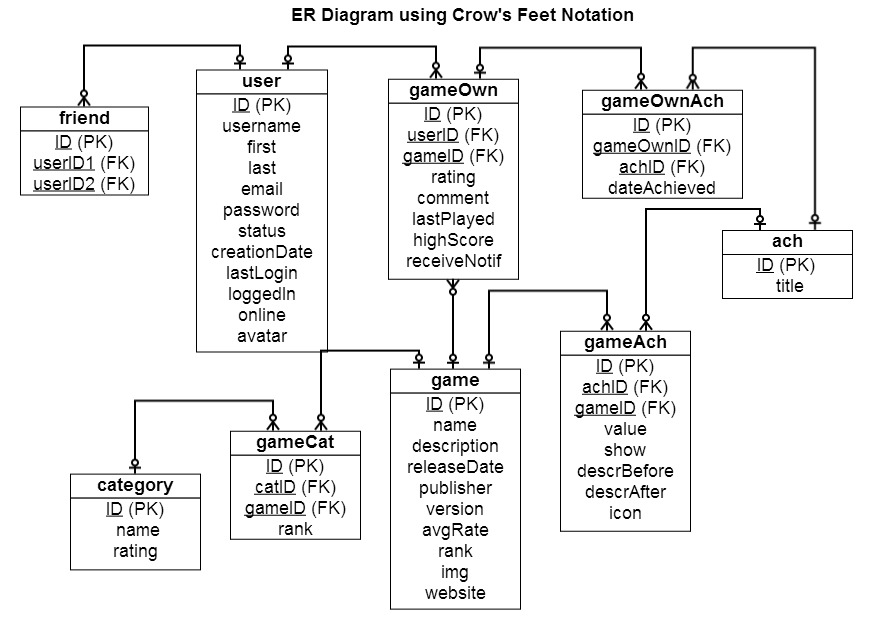
\includegraphics[width=0.80\columnwidth]{er} % Import image
\end{center}

\chapter{\textbf{Appendix B: Data Types}}
\begin{center}
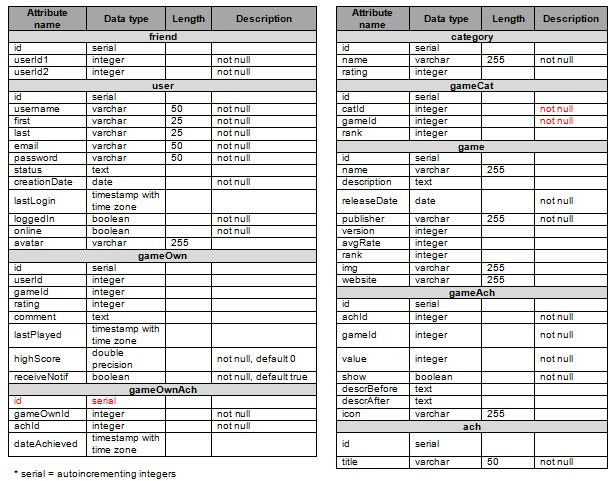
\includegraphics[width=0.80\columnwidth]{types} % Import image
\end{center}

\chapter{\textbf{Appendix C: Mark Allocation}}
\begin{center}
    \begin{tabular}{| l | c | c |}
    \hline
    \textbf{Name} & \textbf{Allocated Mark} & \textbf{Signature} \\ \hline
    Liban Abdulkadir & 0.25 & L.A \\ \hline
    Ana Dumitra\c{s} & 0.25 & A.D \\ \hline
    Andra Irimia & 0.25 & A.I \\ \hline
    Ioan Troan\v{a} & 0.25 & I.T \\ \hline
    \end{tabular}
\end{center}

% To have just one problem per page, simply put a \clearpage after each problem

%\begin{homeworkProblem}
%Listing \ref{homework_example} shows a Perl script.

%\perlscript{homework_example}{Sample Perl Script With Highlighting}

%\lipsum[1]
%\end{homeworkProblem}

%----------------------------------------------------------------------------------------
%	PROBLEM 2
%----------------------------------------------------------------------------------------

%\begin{homeworkProblem}
%\lipsum[2]

%\problemAnswer{
%\begin{center}
%\includegraphics[width=0.75\columnwidth]{example_figure} % Example image
%\end{center}

%\lipsum[3-5]
%}
%\end{homeworkProblem}

%----------------------------------------------------------------------------------------

\end{document}